%-------------------------------------------------
%
% 浙江工业大学硕士学位论文latex模版
% 由于学校论文模版每年会有所变化,使用前请对照调整
%-------------------------------------------------


\documentclass{zjutthesis} % 自定义thesis



\fillmytitle{基于图映射的电磁信号分类方法研究} % 论文题目
\fillmyTITLE{Research on Electromagnetic Signal Classification Method Based on Graph Mapping}% 英文题目
\fillKeywords{调制识别,目标识别,谐波雷达,图映射算法,对比学习 }%关键词
\fillPageNums{60}%论文总页数

%--------------------------------
% 盲审时需要注释掉的的信息
%--------------------------------
\fillAuthorCn{白松航} %作者姓名
\fillAuthorEn{Songhang Bai} %第二页by后的姓名
\fillAuthorNum{221122030217}%学号

\fillsupervisor{翔云} %指导教师姓名
\fillsupervisorTitle{讲师} %指导教师职称
\fillSecondsupervisor{宣琦} %第二导师姓名
\fillSecondsupervisorTitle{教授} %第二导师职称
\fillsupervisorEn{Xiang Yun} %第二页的指导老师姓名
\fillsupervisorTitleEn{Lect.} %第二页的指导老师职称
\fillSecondsupervisorEn{Xuan Qi} %第二页的指导老师姓名
\fillSecondsupervisorTitleEn{Prof.} %第二页的指导老师职称

% 答辩委员会
\fillchairman{徐东伟}%答辩主席的名字
% \fillReviewer{}%评阅人
\fillReviewerMember{陈晋音、陆子平}%答辩委员会成员
%--------------------------------
%--------------------------------

\fillStudyYears{3}%学制几年
\fillMajor{控制工程}  %学科专业
\fillAcademic{工程} %学位类型
\fillDegree{硕士} %学位级别
\fillCultiviate{全日制专业型硕士研究生} %研究生类别
\fillCollege{信息工程学院} %所在学院
\fillresearchArea{信号识别} %研究方向

%答辩时间
\fillDefenseYear{2025} %答辩时间
\fillDefenseMonth{05}
\fillDefenseDay{19}
%提交时间
\fillSubmitYear{2025} %答辩时间
\fillSubmitMonth{06}
\fillSubmitDay{19}


\begin{document} 
    %--------------------------------------------
    % 友情提示:为了加快编译速度,可以注释掉一些章节。最后一起编译
    %--------------------------------------------
    %-------------------------------------------------
% FileName: frontinfo.tex
% Version: 0.1
% Date: 2023-06-25
% Description: 封面
% Others: 
% History: origin
%------------------------------------------------- 

% 根据个人信息修改{}中的内容------------------------

\mytitle{基于图映射的电磁信号分类方法研究} % 论文题目
\myTITLE{Research on Electromagnetic Signal Classification Method Based on Graph Mapping}% 英文题目
\fillAuthorCn{白松航} %作者姓名
\supervisor{翔云} %指导教师姓名
\supervisorTitle{讲师} %指导教师职称
\Secondsupervisor{宣琦} %第二导师姓名
\SecondsupervisorTitle{教授} %第二导师职称
\fillMajor{控制工程}  %学科专业
\fillAcademic{工学硕士} %学位类型
\fillCultiviate{全日制专业型硕士研究生} %研究生类别
\fillCollege{信息工程学院} %所在学院

\fillYear{2025}
\fillMonth{06}
\fillDay{07}

\fillAuthorEn{Songhang Bai} %第二页by后的姓名
\supervisorEn{Xiang Yun} %第二页的指导老师姓名
\supervisorTitleEn{Lect.} %第二页的指导老师职称
\SecondsupervisorEn{Xuan Qi} %第二页的指导老师姓名
\SecondsupervisorTitleEn{Prof.} %第二页的指导老师职称

\fillresearchArea{信号识别} %研究方向
\fillchairman{}%答辩主席的名字


% 指导单位 
% \institute{计算机学院} 
% 完成时间 
%\completedate{2020年4月19日} 

% 以下不用改动-------------------------------------
% 加入书签, bm@frontpage要唯一
\currentpdfbookmark{\deffrontpage}{bm@frontpage}
% 封面无页眉页脚
\thispagestyle{empty}

%----------------------------------------%
% 根据以上的参数 生成标题页,不用修改
%----------------------------------------%

{
    %中文封面
    \begin{center}%gdy++
        {
          
\includegraphics[width=25mm]{logo/zjutlogo}
          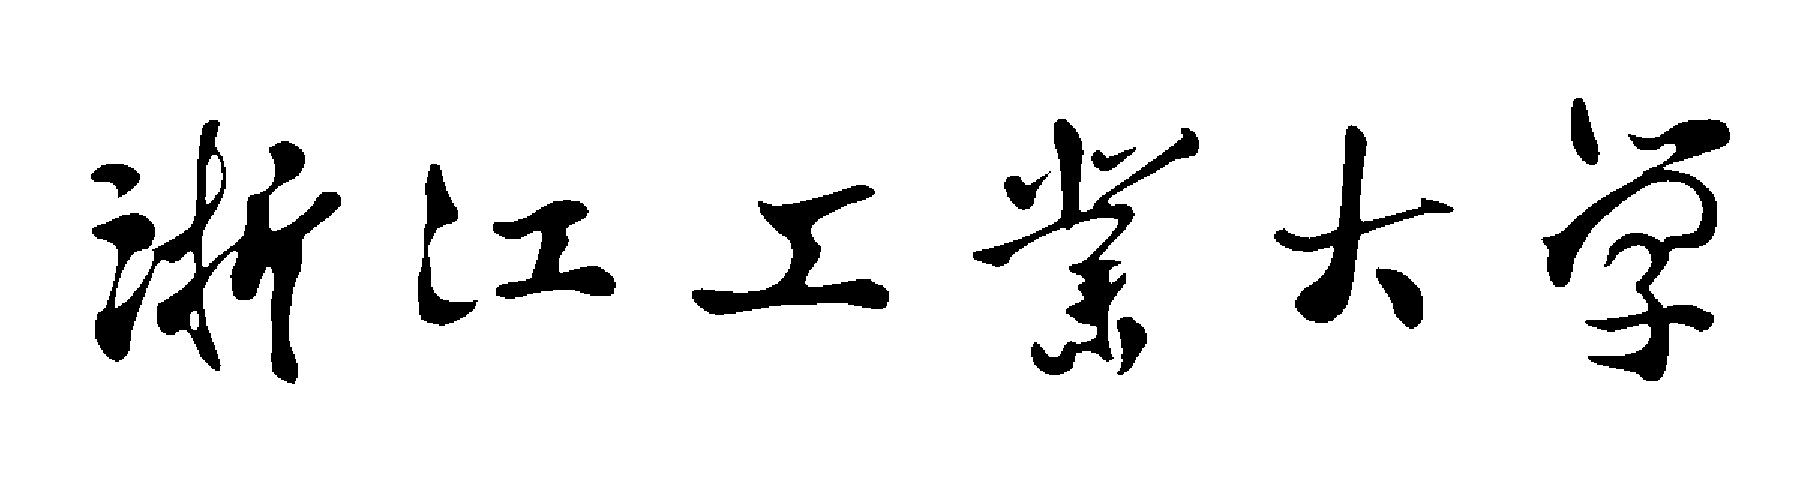
\includegraphics[width=90mm]{logo/zjutname}
        }\\
        \heiti
    
        \vspace*{0.5cm}
        
        {\zihao{0}硕士学位论文}\\
        \vspace*{\fill}
        \begin{tabular}{rc}
          \zihao{3}\defTitleCn \\
        \end{tabular}\\
        \vspace*{3.0cm}
        
        
        \kaiti\bfseries
        \setlength{\tabcolsep}{10mm}{
        \begin{tabular}{rc}
        
          \vspace*{0.3cm}
          \zihao{4}作者姓名 & \zihao{4}\fillAuthorCn \\
          \vspace*{0.3cm}
          \zihao{4}指导教师 & \zihao{4}\defSupervisor\qquad\defSupervisorTitle \\
          \vspace*{0.3cm}
          \zihao{4}第二导师 & \zihao{4}\defSecondSupervisor\qquad\defSecondSupervisorTitle \\
          \vspace*{0.3cm}
          \zihao{4}学科专业 & \zihao{4}\fillMajor \\
          \vspace*{0.3cm}
          \zihao{4}学位类型 & \zihao{4}\fillAcademic \\
          \vspace*{0.3cm}
          \zihao{4}培养类型 & \zihao{4}\fillCultiviate \\
          \vspace*{0.3cm}
          \zihao{4}所在学院 & \zihao{4}\fillCollege \\
        \end{tabular}\\
        }
        %}
        
        \vspace*{\fill}
        {提交日期:\fillYear 年\fillMonth 月}\\
        \vspace*{\fill}
        \end{center}
        \clearpage%{\pagestyle{empty}}
        \thispagestyle{empty}
    %英文封面
        \begin{center}
            \vspace*{1cm}
            {\zihao{1}\sffamily\defTitleEn}\\
            \vspace*{0.5cm}
            \zihao{3}
            Dissertation Submitted to\\
            \textbf{Zhejiang University of Technology}\\
            in partial fulfillment of the requirement\\
            for the degree of\\
            \textbf{Master of Engineering}\\
            
\includegraphics[width=3cm]{logo/zjutlogo}\\
            by\\
            \fillAuthorEn\\
            \vspace*{\fill}
            \begin{tabular}{rl}
                Dissertation Supervisor:&\quad\defSupervisorTitleEn\,\defSupervisorEn\\
            Associate Supervisor:&\quad\defSecondSupervisorTitleEn\,\defSecondSupervisorEn\\
            \end{tabular}
            
            \vspace*{\fill}
            \monthname, \fillYear\\
            \vspace*{\fill}
        \end{center}
        \clearpage%{\pagestyle{empty}}
        \thispagestyle{empty}
        %%gdy--
        
}

       % 封面 (模板根据以上填写的信息生成,不用修改)
    %-------------------------------------------------
% FileName: declaration.tex
% Version: 0.1
% Date: 2023-06-25
% Description: 声明
% Others: 如无需要,不用修改本文件
% History: origin
%-------------------------------------------------

% 断页
\clearpage
% 加入书签, bm@declarationpage要唯一
\currentpdfbookmark{\defdeclarationpage}{bm@declarationpage}
% 封面无页眉页脚
\thispagestyle{empty}

%-----------------------------------------%
% 不用修改
%-----------------------------------------%
% 把一些格式设置的作用范围限制在{}内
{ 
    %原创声明
    \vspace*{24bp}
    \begin{center}
      \zihao{3}\heiti\textbf{浙江工业大学学位论文原创性声明}
    \end{center}
    
    \doublespacing\zihao{-4}
    本人郑重声明:所提交的学位论文是本人在导师的指导下,独立进行研究工作所取得的研究成果。
    除文中已经加以标注引用的内容外,本论文不包含其他个人或集体已经发表或撰写过的研究成果,
    也不含为获得浙江工业大学或其它教育机构的学位证书而使用过的材料。
    对本文的研究作出重要贡献的个人和集体,均已在文中以明确方式标明。
    本人承担本声明的法律责任。
    
    作者签名:\hfill 日期:\defYear 年\defMonth 月 \hspace*{6em}
    
    \vspace*{24bp}
    \begin{center}
    \zihao{3}\heiti\textbf{学位论文版权使用授权书}
    \end{center}
    
    \doublespacing\zihao{-4}
    本学位论文作者完全了解学校有关保留、使用学位论文的规定,
    同意学校保留并向国家有关部门或机构送交论文的复印件和电子版,允许论文被查阅和借阅。
    本人授权浙江工业大学可以将本学位论文的全部或部分内容编入有关数据库进行检索,
    可以采用影印、缩印或扫描等复制手段保存和汇编本学位论文。
    
    \begin{table}[!h]
        \zihao{-4}
      \renewcommand\arraystretch{1.5}
      \begin{tabular}{ll}
        \hspace{1.5em}本学位论文属于 & 1、保密$\square$,在一年解密后适用本授权书。\\
        & 2、保密$\square$,在二年解密后适用本授权书。 \\
        & 3、保密$\square$,在三年解密后适用本授权书。 \\
        & 4、不保密$\square$。 \\
        & (请在以上相应方框内打“√”) \\
      \end{tabular}
    \end{table}
    
    作者签名:\hfill 日期:\defYear 年\defMonth 月 \hspace*{6em}
    
    导师签名:\hfill 日期:\defYear 年\defMonth 月 \hspace*{6em}
    
    \clearpage%{\pagestyle{empty}}
    \thispagestyle{empty}
    %论文分类号
    \begin{tabular*}{0.93\hsize}{@{\extracolsep{0.6cm}}r l c r l}   %   这里面的@什么意思
        %\hline
        \zihao{5}中图分类号                   & \zihao{5}TP391       &     &        \zihao{5}学校代码   &     \zihao{5}10337                           \\ %\hline
        \zihao{5}UDC 					& \zihao{5}004.8 			& 	& 		\zihao{5}密级				&\zihao{5}公开						\\  
        \vspace{0.5cm} %\hline
        \zihao{5}研究生类别				& \zihao{5}\defCultiviate  &   &     &    \\
    \end{tabular*}	
    {\centering
        {
            
\includegraphics[width=15mm]{logo/zjutlogo}
            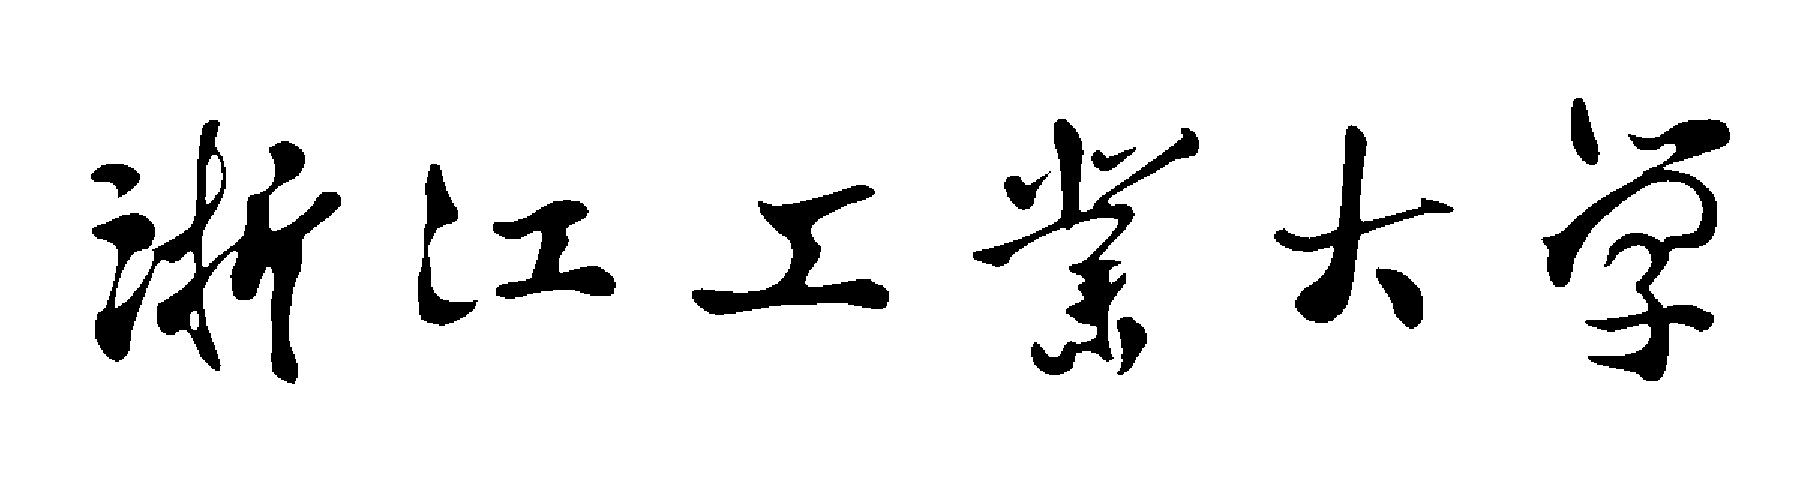
\includegraphics[width=65mm]{logo/zjutname}
            
            \vspace*{0.1cm}
            \heiti{\zihao{2}硕士学位论文}\\
            \vspace*{2cm}
            \zihao{3}\defTitleCn \\
            \vspace*{0.4cm}
            \zihao{3}\defTitleEn \\
        }       %\leavevmode
        
        \vspace*{3cm}
    }

    \zihao{4}
    \begin{tabular*}{0.88\hsize}{@{\extracolsep{\fill}}l b{3.6cm} c l b{3.8cm}}   %   这里面的@什么意思
        %\hline
        作者姓名         & \defAuthorCn                &    &      第一导师  &     \defSupervisor\hspace{0.2cm}\defSupervisorTitle \\
        
        申请学位 &  \defAcademic 	&	&    第二导师 & 
         \defSecondSupervisor\hspace{0.2cm}\defSecondSupervisorTitle		\\  
        学科专业		& \defMajor  &   &   培养单位& \defCollege   \\
    %\end{tabular*}	\\
    %\begin{tabular*}{0.88\hsize}{@{\extracolsep{\fill}}l b{3.6cm} c l b{3.8cm}} 
        研究方向 &  \defResearchArea	&	& 		答辩委员会主席	&  \defChairman		\\ 
        
    \end{tabular*}	\\
    
    \vspace*{3cm}
    {\centering
        \zihao{4}
        {	
            \begin{tabular*}{0.8\hsize}{@{\extracolsep{\fill}}ccc c ccc}   %   这里面的@什么意思
                %\hline
                \hspace{1.0cm} 答辩日期:        & \defYear      &  年   &       \defMonth  &     月      & \defDay &     日\hspace{1.8cm}       \\ %\hline
            \end{tabular*}	\\
        }
    }

}    



     % 声明 (不用修改)
    %-------------------------------------------------
% FileName: abstract-ch.tex
% Version: 0.1
% Date: 2023-06-25
% Description: 中文摘要
% Others: 
% History: origin
%------------------------------------------------- 

% 以下不用改动-------------------------------------
% 断页
\clearpage
% 页码从1开始计数
\setcounter{page}{1}
% 大写罗马数字显示页码
\pagenumbering{Roman}
% 加入书签, bm@abstractname要唯一
\phantomsection %创建跳转锚点 否则会跳转错误
\addcontentsline{toc}{chapter}{\defabstractname}
% \currentpdfbookmark{\defabstractname}{bm@abstractname}
% \chapter*{} 表示不编号,不生成目录
% \markboth{}{} 用于页眉
% 此处以中文题目作为章题目 星号*表示不编号
\chapter*{\defTitleCn}


% 修改摘要和关键词---------------------------------
% 中文摘要
\abstract{
摘要反映了毕业设计(论文)的主要信息,以浓缩的形式概括说明研究目的、内容、方法、成果和结论,具有独立性和完整性。中文摘要一般为400字左右,不含公式、图表和注释。论文摘要应采用第三人称的写法,力求文字精悍简练。

摘要要交代清楚毕业设计的几个问题:why,what,how,results和meaningful。Why为什么要设计这个作品,通常是为了解决某个问题,比如现有的设计有缺陷,或者用户有某些需要。What完成了一个什么样的作品,具备哪些功能。How怎么完成这个作品的,用了哪些技术,一些关键功能模块是怎么设计和实现的。Results和meaningful有什么结果和意义,通常去回答开始提出的why,作品确实解决了某个问题,或者取得了某个效果。
}

% 中文关键词
% 关键词是供检索用的主题词条,应采用能覆盖毕业设计(论文)主要内容的通用技术词条(参照相应的技术术语标准)。关键词一般为3~5个,每个关键词不超过5个字。
\keywords{毕业设计;作品;技术;结果;意义}


     % 中文摘要
    %-------------------------------------------------
% FileName: abstract-en.tex
% Version: 0.1
% Date: 2023-06-25
% Description: 英文摘要
% Others: 
% History: origin
%------------------------------------------------- 

% 以下不用改动-------------------------------------
% 断页
\clearpage
% 加入书签, bm@ABSTRACTNAME要唯一
\phantomsection %创建跳转锚点 否则会跳转错误
\addcontentsline{toc}{chapter}{\defABSTRACTNAME}
% \addcontentsline{toc}{chapter}{Abstract}
% \chapter*{} 表示不编号,不生成目录
% \markboth{}{} 用于页眉
% 此处以英文题目作为章题目
\chapter*{\defTitleEn}

% 修改摘要和关键词---------------------------------
% 英文摘要
% 英文摘要与中文摘要的内容应一致。
\ABSTRACT{
Fourscore and seven years ago, our fathers brought forth upon this continent a new Nation, conceived in Liberty, and dedicated to the proposition that all men are created equal. Now, we are engaged in a great Civil War, testing whether that Nation, or any nation so conceived and so dedicated, can long endure. We are met on a great battlefield of that war. We have come to dedicate a portion of that field as a final resting-place for those who here gave their lives that that Nation might live. It is altogether fitting and proper that we should do this.

But, in a larger sense, we cannot dedicate, we cannot consecrate, we cannot hallow this ground. The brave men, living and dead, who struggled here, have consecrated it far above our poor power to add or detract. The world will little note nor long remember what we say here, but it can never forget what they did here. It is for us, the living, rather to be dedicated here to the unfinished work which they who fought here have thus far so nobly advanced. It is rather for us to be here dedicated to the great task remaining before us; that from these honored dead, we take increased devotion to that cause for which they gave the last full measure of devotion; that we here highly resolve that these dead shall not have died in vain, that this Nation, under GOD, shall have a new birth of freedom; and that government of the People by the People and for the People shall not perish from the earth.
}

% 英文关键词
% 每一个英文关键词都必须与中文关键词一一对应。
\KEYWORDS{Thesis; Hello world; Good luck; Congratulations}




 

     % 英文摘要
    %-------------------------------------------------
% FileName: content.tex
% Version: 0.1
% Date: 2023-06-25
% Description: 目录
% Others: 如无需要,不用修改本文件
% History: origin
%-------------------------------------------------

% 断页
\clearpage
% 加入书签, bm@contentsname要唯一
\phantomsection
\addcontentsline{toc}{chapter}{目录}
% 生成目录

\tableofcontents 

% 断页
\clearpage
% 加入书签, bm@listfigurename要唯一
\phantomsection
\addcontentsline{toc}{chapter}{插图清单}
% 生成图目录
\listoffigures



% 断页
\clearpage
% 加入书签, bm@listtablename要唯一
\phantomsection
\addcontentsline{toc}{chapter}{附表清单}
% 生成表目录
 \listoftables



         % 目录 (如无需要,不用修改)
    %-------------------------------------------------
% FileName: chapt-1.tex
% Version: 0.1
% Date: 2023-06-25
% Description: 第1章
% Others: 
% History: origin
%------------------------------------------------- 

% 断页
\clearpage
% 页码从1开始计数
\setcounter{page}{1} 
% 阿拉伯数字显示页码
\pagenumbering{arabic}

\chapter{绪论}

% 这里的\label是为了下面的交叉引用
\section{课题背景}\label{sec:background}
简要介绍本文的开发背景。明确说明哪些是别人已经做过的工作,哪些是自己要做的工作。

% 分段是通过空行来实现的
话说得远一点,正是因为很多人不接受休谟的这个观点,才使得文艺创作者们有各种花招可以玩。比如《黑客帝国》后两集里的招数:让观众怀疑反抗军的基地也是虚拟出来的。比如《盗梦空间》里,让观众怀疑所谓的真实世界还是一个梦境。

% 引用多篇参考文献 [1-3]
贪婪是人的本性,也是资本主义社会发展的必不可少的动力。但是今天的资本主义社会学会了用很多方法去克制个人贪欲。比如通过宗教的约束,比如通过立法的形式,遏制垄断企业(可怜的微软),遏制不正当和不道德的竞争,给工人更多的福利\cite{chen2005laser, mittelbach2004latex, zhen2018leave}。

% 有序列表嵌套
唐诗,宋词,元曲举例:
\begin{enumerate}
	\item 唐诗
	\begin{enumerate} 
		% \item 蜀道难(李白)噫吁嚱,危乎高哉!蜀道之难,难于上青天!蚕丛及鱼凫,开国何茫然!尔来四万八千岁,不与秦塞通人烟。西当太白有鸟道,可以横绝峨眉巅。地崩山摧壮士死,然后天梯石栈相钩连。上有六龙回日之高标,下有冲波逆折之回川。黄鹤之飞尚不得过,猿猱欲度愁攀援。青泥何盘盘,百步九折萦岩峦。扪参历井仰胁息,以手抚膺坐长叹。
		\item 春晓(孟浩然)春眠不觉晓,处处闻啼鸟。夜来风雨声,花落知多少。
	\end{enumerate}
	\item 宋词
	\begin{enumerate}
		\item 破阵子(辛弃疾)醉里挑灯看剑,梦回吹角连营。八百里分麾下炙,五十弦翻塞外声,沙场秋点兵。马作的卢飞快,弓如霹雳弦惊。了却君王天下事,赢得生前身后名。可怜白发生!
		\item 赤壁怀古(苏轼)大江东去,浪淘尽,千古风流人物。故垒西边,人道是,三国周郎赤壁。乱石穿空,惊涛拍岸,卷起千堆雪。江山如画,一时多少豪杰。遥想公瑾当年,小乔初嫁了,雄姿英发。羽扇纶巾,谈笑间,樯橹灰飞烟灭。故国神游,多情应笑我,早生华发。人生如梦,一尊还酹江月。
	\end{enumerate}
	\item 元曲
	\begin{enumerate}
		\item 窦娥冤(关汉卿)花有重开日,人无再少年。不须长富贵,安乐是神仙。老身蔡婆婆是也。楚州人氏,嫡亲三口儿家属。不幸夫主亡逝已过,止有一个孩儿,年长八岁。俺娘儿两个,过其日月。家中颇有些钱财。这里一个窦秀才,从去年问我借了二十两银子,如今本利该银四十两。我数次索取,那窦秀才只说贫难,没得还我。他有一个女儿,今年七岁,生得可喜,长得可爱。我有心看上他,与我家做个媳妇,就准了这四十两银子,岂不两得其便!他说今日好日辰,亲送女儿到我家来。老身且不索钱去,专在家中等候。这早晚窦秀才敢待来也。
		\item 秋思(马致远)枯藤老树昏鸦,小桥流水人家,古道西风瘦马。夕阳西下,断肠人在天涯。
	\end{enumerate}
\end{enumerate}

% 这里的\label是为了下面的交叉引用
\section{目的意义}\label{sec:meaningful}
介绍本课题的研究意义、研究目的、主要研究内容、研究范围和应该解决的问题。

% 下面演示怎么增加子标题
\subsection{目的意义1}
\subsubsection{目的意义11}


\section{论文主要工作}
介绍本研究课题的来源及主要研究内容。

% 下面是一个引用节的例子
论文的背景见\ref{sec:background},论文的目的意义见\ref{sec:meaningful}。

本作品分工如下,虚若无同学实现:
% 下面是一个无序列表的例子
\begin{itemize}
	\item 系统架构设计;
	\item 功能模块的设计与实现;
	\item web端的编程与实现;
	\item 数据库设计。
\end{itemize}
          % 第1章
    %-------------------------------------------------
% FileName: chapt-2.tex
% Version: 0.1
% Date: 2023-06-25
% Description: 第2章
% Others: 
% History: origin
%------------------------------------------------- 

% 断页
% \clearpage
\chapter{相关技术和理论基础}



\section{质能方程}
行内公式,用两个\$:质能方程即描述质量与能量之间的当量关系的方程\cite{liuxiaopingwordandtex}。质能方程$e=mc^2$,$e$表示能量,$m$代表质量,而$c$则表示光速,由爱因斯坦提出\cite{yassin1994latex}。

\section{牛顿力学}
% 下面说明公式的引用。
公式引用:任何物体都要保持匀速直线运动或静止状态\cite{liu2013latex},直到外力迫使它改变运动状态为止,见公式\eqref{eq:newton}。
% 行间公式,用环境 equation
% \label用于标注公式,在别处引用
\begin{equation}\label{eq:newton}
	\vec{F}=m\vec{a} 
\end{equation}




    %-------------------------------------------------
% FileName: chapt-3.tex
% Version: 0.1
% Date: 2023-06-25
% Description: 第3章
% Others: 
% History: origin
%------------------------------------------------- 

% 断页
% \clearpage 

\chapter{系统分析(需求分析)}

\section{功能需求分析}
% 引用图片的例子
描述系统的功能性需求,可以通过数据流图或UML的用例图等图表工具来部来定义系统的功能需求,并把需求和设计完全分离开。如图\ref{fig:single}所示。

% xelatex 支持的图片格式
% 矢量图 .pdf .eps 
% 位图 .jpg .png .bmp

% figure环境
% [H] 浮动优先级,当前位置,但尺寸过大的浮动体可能使得分页比较困难

% [htbp!] 浮动方式 请参考一份(不太)简短的 LATEX 2" 介绍,3.9节
% h 当前位置(代码所处的上下文)
% t 顶部
% b 底部
% p 单独成页
% ! 在决定位置时忽视限制
% 排版位置的选取与参数里符号的顺序无关, 
% LATEX 总是以 h-t-b-p 的优先级顺序决定浮动体位置。
% 也就是说 [!htp] 和 [ph!t] 没有区别。

\begin{figure}[H]
	% 居中
	\centering 
	% width=.5\textwidth 文档宽度的0.5
	% fig1图片放在img目录下,在此处引用无需img/前缀和图片格式后缀(png, jpg等)
	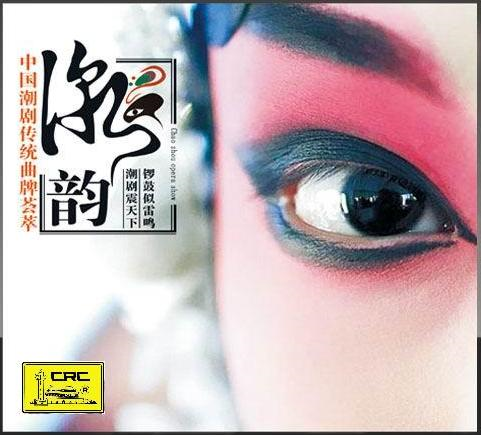
\includegraphics[width=.5\textwidth]{fig1} 
	% label紧接caption之后,用于引用
        \bicaption{这是一个很长很长的图}{This is a long tu}
	\label{fig:single}
\end{figure}


 
 


           % 增加新章节到tex目录,此处input
    %-------------------------------------------------
% FileName: chapt-4.tex
% Version: 0.1
% Date: 2023-06-25
% Description: 第4章
% Others: 
% History: origin
%------------------------------------------------- 


% 断页
% \clearpage
\chapter{系统设计}

\section{总体设计}
描述根据系统的需求分析,确定系统的功能模块构成。

\section{详细设计}
说明各个功能模块的数据结构和实现算法。


C源代码
\begin{clan}
    #include <stdio.h>  
    int main()                  //main 入口函数  
    {  
        printf("Hello,World!"); //printf 函数打印  
        return 1;               //函数返回值  
    }   
\end{clan}


matlab源代码
    \begin{matlab}
    function F=random()
    a=[1 2];
    Prob=[0.99 0.01];
    F=randsrc(1,1,[a;Prob]);

    areas=[]
    for i=1:100
    x=unifrnd(0,10,[1,100]);
    y=unifrnd(0,10,[1,100]);
    frequency=sum(x<=1)+sum(y<=1);
    area=100*frequency/100;
    areas=[areas,area];
    end
\end{matlab}


python源代码
\begin{python}
    from multiprocessing import Pool
    import os, time, random

    def long_time_task(name):
        print('Run task %s (%s)...' % (name, os.getpid()))
        start = time.time()
        time.sleep(random.random() * 3)
        end = time.time()
        print('Task %s runs %0.2f seconds.' % (name, (end - start)))

    if __name__=='__main__':
        print('Parent process %s.' % os.getpid())
        p = Pool(4)
        for i in range(5):
        p.apply_async(long_time_task, args=(i,))
        print('Waiting for all subprocesses done...')
        p.close()
        p.join()
        print('All subprocesses done.')
\end{python}




C++源代码
\begin{cpp}
    #include <iostream>               //std::cout 要用到的头文件  
    #include <stdio.h>                //标准输入输出头文件  

    int main()  
    {  
        printf("Hello,World!--Way 1\n");    //printf 语句打印  
        puts("Hello,World!--Way 2");        //puts 语句  
        puts("Hello," " " "World!--Way 3"); //字符串拼接  
        std::cout << "Hello,World!--Way 4" << std::endl; //C++ 教科书上写法  
        return 1;                                        //作为注释  
    }  
\end{cpp}




Csharp源代码
\begin{clan}
    //FileName: HelloWorld.cs  
    using System;  
    class TestApp  
    {  
        public static void Main()  
        {  
            Console.WriteLine("Hello,World!");  
            Console.ReadKey();  
        }  
    }   
\end{clan}

java源代码
\begin{java}
    #FileName: HelloWorld.java 
    #如果有 public 类的话,类名必须和文件同名,注意大小写   
    public class HelloWorld   
    {  
        #Java 入口程序,程序从此入口  
        public static void main(String[] args)  
        {  
            #向控制台打印一条语句  
            System.out.println("Hello,World!");  
        }  
    }  
\end{java}


js源代码
\begin{javascript}
    var sys = require("sys");    #导入需要的 sys 模块  
    sys.puts("Hello,World!");    #调用里面的 puts 函数来打印字符串  
\end{javascript}

php源代码
\begin{php} 
    <?php  
        echo "Hello,World!";            //打印语句  
        echo "The first php program!";  //打印语句  
        echo phpinfo();                 //phpinfo()系统函数,输出环境信息  
    ?>    
\end{php}


go源代码
\begin{gogo}

    //filename: hello.go
    package main 
    import (
        "fmt"
        "os"
    )
    func main(){ //这个 { 不能另起一行
        fmt.Println("hello world!")
    }
\end{gogo}

html源代码
\begin{html}
    <!DOCTYPE html>  
    <html>  
        <body>  
            <h1>This is the first program!</h1>  
            <p>Hello,World!</p>  
        </body>  
    </html>
\end{html}

xml源代码 
\begin{xml}
    <?xml version="1.0"?>
    <class name="Student" table="student">
        <id name="id" column="id" ></id>
        <property name="name" column="name" ></property>
        <property name="age" column="age" ></property>
    </class> 
\end{xml}

sql源代码 
\begin{sql}
    SQL> CREATE TABLE MESSAGE (TEXT CHAR(15));            #创建表  
    INSERT INTO MESSAGE (TEXT) VALUES ('Hello, world!');  #插入表  
    SELECT TEXT FROM MESSAGE;                             #查询表  
    DROP TABLE MESSAGE;                                   #删除表               
    Table created.   
\end{sql}

tex源代码 
\begin{tex}
    \begin{figure}[H]
        % 居中
        \centering 
        % width=.5\textwidth 文档宽度的0.5
        % fig1图片放在img目录下,在此处引用无需img/前缀和图片格式后缀(png, jpg等)
        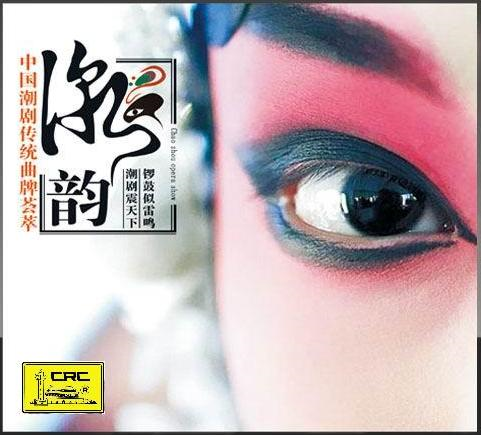
\includegraphics[width=.5\textwidth]{fig1} 
        % label紧接caption之后,用于引用
        \caption{这是一个图}
        \label{fig:single2}
    \end{figure}
\end{tex} 
    %-------------------------------------------------
% FileName: chapt-5.tex
% Version: 0.1
% Date: 2023-06-25
% Description: 第5章
% Others: 
% History: origin
%------------------------------------------------- 


% 断页
% \clearpage
\chapter{系统实现与测试}

\section{系统实现}
介绍主要功能模块的编程实现以及系统的部署方法。

\section{系统测试}
阐述系统的测试技术、测试过程和测试结果。
\begin{figure}[H]
	% 居中
	\centering 
	% width=.5\textwidth 文档宽度的0.5
	% fig1图片放在img目录下,在此处引用无需img/前缀和图片格式后缀(png, jpg等)
	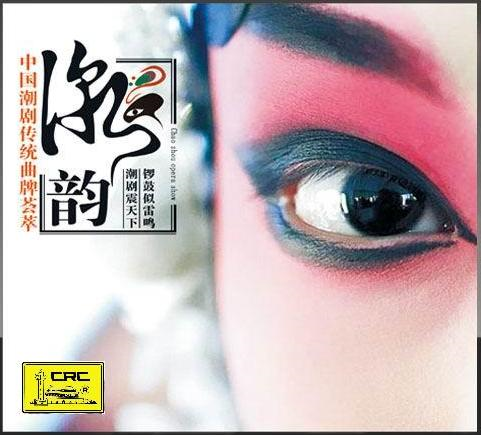
\includegraphics[width=.5\textwidth]{fig1} 
	% label紧接caption之后,用于引用
        \bicaption{这是一个很长很长的图}{This is a long tu}
	\label{fig:single3}
\end{figure}
完全手动完成的表格,如表\ref{tab:tab1}所示。
\begin{table}[h] % htbp 浮动优先级
	\centering  % 居中
	% \caption{一个表格}  % 表格标题
        \bicaption{一个表格}{a table}
	\label{tab:tab1}  % 用于引用的label
	% 字母的个数对应列数,|代表分割线
	% l代表左对齐,c代表居中,r代表右对齐
	\begin{tabular}{|c|c|c|c|}   
		\hline  % 表格的横线 
		1 & 2 & 3 & 4 \\  % 表格中的内容,用&分开,\\表示下一行
		\hline 
		0.1 & 0.2 & 0.3 & 0.4 \\
		\hline
	\end{tabular}
\end{table}

    %-------------------------------------------------
% FileName: chapt-6.tex
% Version: 0.1
% Date: 2023-06-25
% Description: 第6章
% Others: 
% History: origin
%------------------------------------------------- 

% 断页
% \clearpage

\chapter{总结和展望 }
是对整个毕业设计工作的归纳和综合,对现有成果和尚存在的问题的描述,以及进一步开展研究的见解与建议。

\section{本文总结}
 
\section{未来展望}
 



% \begin{lstlisting}[language=TeX,frame=single,]
% { 
%   $\int f(x) \mathrm{d}x$
%   $\sum_{0}^{+\infty}$
%   \begin{center}
%   居中
%   \end{center}
% }
% \end{lstlisting}

          
    %-------------------------------------------------
% FileName: reference.tex
% Version: 0.1
% Date: 2023-06-25
% Description: 参考文献
% Others: 如无需要,不用修改本文件
%         参考文献请到 bib/ref.bib中按格式增加
% History: origin
%-------------------------------------------------


% 参考文献是毕业设计(论文)不可缺少的组成部分,在毕业设计(论文)的撰写过程中应承认和尊重他人的知识成果,参考与引用的内容必须注明,杜绝抄袭、剽窃他人成果。同时,引用的资料应具有权威性,并对毕业设计(论文)有直接的参考价值。
% 要求查阅文献15篇(含)以上,其中外文文献3篇(含)以上,近三年公开发表的文献3篇(含)以上,书籍不超过5本,期刊([J])和论文集([C])8篇(含)以上,包括导师指定的全部参考文献。


% 断页
\clearpage

% hyperef 精确定位
% 设置一个anchor,主要针对\addcontentsline
% 防止目录,书签等指向错误位置 
\phantomsection

% 增加到目录,与chapter同级别
\addcontentsline{toc}{chapter}{\bibname}

%------------------------------------------
% 默认参考文献样式 plain
% \bibliographystyle{plain}
% gbt7714 顺序编码制
\bibliographystyle{bib/gbt7714-numerical} 
%------------------------------------------

% ref是BIBTEX数据库的文件名,不要带.bib 扩展名,实际文件 bib/ref.bib
\bibliography{bib/ref}

% 把所有未引用的文献也列出
% \nocite{*} 



         % 参考文献 (修改bib/ref.bib)
    %-------------------------------------------------
% FileName: acknowledgement.tex
% Version: 0.1
% Date: 2023-06-25
% Description: 致谢
% Others: 
% History: origin
%------------------------------------------------- 

% 以下不用改动-------------------------------------
% 断页
\clearpage
% hyperef 精确定位
% 设置一个anchor,主要针对\addcontentsline
% 防止目录,书签等指向错误位置 
\phantomsection
%增加到目录,与chapter同级别
\addcontentsline{toc}{chapter}{\defacknowledgement}
% \chapter*{} 表示不编号,不生成目录
% \markboth{}{} 用于页眉
\chapter*{\defacknowledgement}

% 修改以下内容---------------------------------
% 设置行距1.5
{\linespread{1.5} \selectfont 简述自己通过毕业设计(论文)的体会,向给予指导、合作、支持及协助完成研究工作的单位、组织或个人致谢。致谢的文字虽不多,却是论文不可缺少的内容。内容应简洁明了、实事求是,避免俗套。

第二段致谢。

第三段致谢。\par} %\par 强制换行,使得行距生效

 % 致谢 
    %-------------------------------------------------
% FileName: appendix.tex
% Version: 0.1
% Date: 2023-06-25
% Description: 附录
% Others: 如果没有内容,就在main.tex中注释掉
% History: origin
%------------------------------------------------- 


% 以下不用改动-------------------------------------
% 断页
% \clearpage



% hyperef 精确定位
% 设置一个anchor,主要针对\addcontentsline
% 防止目录,书签等指向错误位置 
% \phantomsection
% 增加到目录,与chapter同级别
% \addcontentsline{toc}{chapter}{\appendixname} 
% \chapter*{} 表示不编号,不生成目录
% \markboth 用于页眉
% \chapter*{\appendixname \markboth{\appendixname}{}} 

% appendix 用于附录章节的特殊编号 从A开始

\newcommand{\name}{作者简介}

% 附录章
% 断页
\clearpage
% hyperef 精确定位
% 设置一个anchor,主要针对\addcontentsline
% 防止目录,书签等指向错误位置 
\phantomsection
%增加到目录,与chapter同级别
\addcontentsline{toc}{chapter}{\name}
% \chapter*{} 表示不编号,不生成目录
% \markboth{}{} 用于页眉
\chapter*{\name \markboth{\name}{}}

% 修改以下内容---------------------------------
此处为作者简介


        % 作者简介 
    \newcommand{\aname}{学术论文数据集}

% 附录章
% 断页
\clearpage
% hyperef 精确定位
% 设置一个anchor,主要针对\addcontentsline
% 防止目录,书签等指向错误位置 
\phantomsection
%增加到目录,与chapter同级别
\addcontentsline{toc}{chapter}{\aname}
% \chapter*{} 表示不编号,不生成目录
% \markboth{}{} 用于页眉
\chapter*{\aname \markboth{\aname}{}}

%特别定义微软雅黑字体,需要字体文件
\setCJKfamilyfont{zhyahei}{MSYH}[Path=fonts/,Extension = .TTC]
\ProvideDocumentCommand \yahei{}{\CJKfamily{zhyahei}}
{
  \setlength{\tabcolsep}{0.1cm}%设置表列间距
  \renewcommand{\arraystretch}{1.5}%设置10行距倍数
  \vspace{-24pt}
  \begin{tcolorbox}[
      sharp corners,
      boxrule=1pt,
      colback=white,
      boxsep=0pt,
      left=0pt,right=0pt,top=0pt,bottom=0pt
    ]
      \yahei %为了简单,统一设置字体
      \resizebox{\textwidth}{!}{%
      \begin{tabular}{|>{\centering\arraybackslash}m{2cm}>{\centering\arraybackslash}m{2cm}>{\centering\arraybackslash}m{2cm}>{\centering\arraybackslash}m{2cm}>{\centering\arraybackslash}m{4cm}>{\centering\arraybackslash}m{2cm}>{\centering\arraybackslash}m{2cm}|}
          \hline
          \multicolumn{2}{|>{\centering\arraybackslash}m{4cm}|}{密\quad 级*}          & \multicolumn{2}{>{\centering\arraybackslash}m{4cm}|}{中图分类号*}            & \multicolumn{1}{>{\centering\arraybackslash}m{4cm}|}{UDC*}          & \multicolumn{2}{>{\centering\arraybackslash}m{4cm}|}{论文资助}      \\ \hline
          \multicolumn{2}{|>{\centering\arraybackslash}m{4cm}|}{公开}            & \multicolumn{2}{>{\centering\arraybackslash}m{4cm}|}{TP391}             & \multicolumn{1}{>{\centering\arraybackslash}m{4cm}|}{004.8}         & \multicolumn{2}{>{\centering\arraybackslash}m{4cm}|}{}          \\ \hline
          \multicolumn{2}{|>{\centering\arraybackslash}m{4cm}|}{学位授予单位名称}      & \multicolumn{2}{>{\centering\arraybackslash}m{4cm}|}{学位授予单位代码}          & \multicolumn{1}{>{\centering\arraybackslash}m{4cm}|}{学位类型*}         & \multicolumn{2}{>{\centering\arraybackslash}m{4cm}|}{学位级别*}     \\ \hline
          \multicolumn{2}{|>{\centering\arraybackslash}m{4cm}|}{浙江工业大学}        & \multicolumn{2}{>{\centering\arraybackslash}m{4cm}|}{10337}             & \multicolumn{1}{>{\centering\arraybackslash}m{4cm}|}{\defAcademic}            & \multicolumn{2}{>{\centering\arraybackslash}m{4cm}|}{硕士}        \\ \hline
          \multicolumn{1}{|>{\centering\arraybackslash}m{2cm}|}{论文题名*} & \multicolumn{6}{>{\centering\arraybackslash}m{14cm}|}{\defTitleCn}                                                                                \\ \hline
          \multicolumn{1}{|>{\centering\arraybackslash}m{2cm}|}{关键词*}  & \multicolumn{5}{>{\centering\arraybackslash}m{12cm}|}{\defKeywords}                                                       & 论文语种*         \\ \hline
          \multicolumn{1}{|>{\centering\arraybackslash}m{2cm}|}{并列题名*} & \multicolumn{5}{>{\centering\arraybackslash}m{12cm}|}{\defTitleEn} & 中文            \\ \hline
          \multicolumn{2}{|>{\centering\arraybackslash}m{4cm}|}{作者姓名*}         & \multicolumn{2}{>{\centering\arraybackslash}m{4cm}|}{\defAuthorCn}                  & \multicolumn{1}{>{\centering\arraybackslash}m{4cm}|}{学\quad 号*}          & \multicolumn{2}{>{\centering\arraybackslash}m{4cm}|}{\defAuthorNum}          \\ \hline
          \multicolumn{2}{|>{\centering\arraybackslash}m{4cm}|}{培养单位名称*}       & \multicolumn{2}{>{\centering\arraybackslash}m{4cm}|}{培养单位代码*}           & \multicolumn{1}{>{\centering\arraybackslash}m{4cm}|}{培养单位地址}        & \multicolumn{2}{>{\centering\arraybackslash}m{4cm}|}{邮政编码}      \\ \hline
          \multicolumn{2}{|>{\centering\arraybackslash}m{4cm}|}{浙江工业大学\defCollege}  & \multicolumn{2}{>{\centering\arraybackslash}m{4cm}|}{10337}             & \multicolumn{1}{>{\centering\arraybackslash}m{4cm}|}{杭州市潮王路18号}     & \multicolumn{2}{>{\centering\arraybackslash}m{4cm}|}{310032}    \\ \hline
          \multicolumn{2}{|>{\centering\arraybackslash}m{4cm}|}{学科专业*}         & \multicolumn{2}{>{\centering\arraybackslash}m{4cm}|}{研究方向*}             & \multicolumn{1}{>{\centering\arraybackslash}m{4cm}|}{学\quad 制*}          & \multicolumn{2}{>{\centering\arraybackslash}m{4cm}|}{学位授予年*}    \\ \hline
          \multicolumn{2}{|>{\centering\arraybackslash}m{4cm}|}{\defMajor}          & \multicolumn{2}{>{\centering\arraybackslash}m{4cm}|}{\defResearchArea}              & \multicolumn{1}{>{\centering\arraybackslash}m{4cm}|}{\defStudyYears}             & \multicolumn{2}{>{\centering\arraybackslash}m{4cm}|}{\defSubmitYear}      \\ \hline
          \multicolumn{2}{|>{\centering\arraybackslash}m{4cm}|}{论文提交日期*}       & \multicolumn{5}{>{\centering\arraybackslash}m{12cm}|}{\defSubmitYear 年\defSubmitMonth 月}                                                                                \\ \hline
          \multicolumn{2}{|>{\centering\arraybackslash}m{4cm}|}{导师姓名*}         & \multicolumn{2}{>{\centering\arraybackslash}m{4cm}|}{\defSupervisor}                  & \multicolumn{1}{>{\centering\arraybackslash}m{4cm}|}{职\quad 称*}          & \multicolumn{2}{>{\centering\arraybackslash}m{4cm}|}{\defSupervisorTitle}          \\ \hline
          \multicolumn{2}{|>{\centering\arraybackslash}m{4cm}|}{评阅人}           & \multicolumn{2}{>{\centering\arraybackslash}m{4cm}|}{答辩委员会主席*}          & \multicolumn{3}{>{\centering\arraybackslash}m{8cm}|}{答辩委员会成员}                                        \\ \hline
          \multicolumn{2}{|>{\centering\arraybackslash}m{4cm}|}{\defReviewer}              & \multicolumn{2}{>{\centering\arraybackslash}m{4cm}|}{\defChairman}                  & \multicolumn{3}{>{\centering\arraybackslash}m{8cm}|}{\defReviewerMember}                                               \\ \hline
          \multicolumn{7}{|>{\raggedright\arraybackslash}p{16cm}|}{电子版论文提交格式:文本(√)图像(\quad)视频(\quad)音频(\quad)多媒体(\quad)其他(\quad)}                                                                          \\ \hline
          \multicolumn{3}{|>{\centering\arraybackslash}m{6cm}|}{电子版论文出版(发布)者}                       & \multicolumn{2}{>{\centering\arraybackslash}m{6cm}|}{电子版论文出版(发布)地}                      & \multicolumn{2}{>{\centering\arraybackslash}m{4cm}|}{版权声明}      \\ \hline
          \multicolumn{3}{|>{\centering\arraybackslash}m{6cm}|}{}                                   & \multicolumn{2}{>{\centering\arraybackslash}m{4cm}|}{}                                  & \multicolumn{2}{>{\centering\arraybackslash}m{4cm}|}{}          \\ \hline
          \multicolumn{2}{|>{\centering\arraybackslash}m{4cm}|}{论文总页数*}        & \multicolumn{5}{>{\centering\arraybackslash}m{12cm}|}{\defPageNums}                                                                                      \\ \hline
          \multicolumn{7}{|>{\raggedright\arraybackslash}p{16cm}|}{注:共33项,其中带*为必填数据,为22项。}                                                                                                       \\
          \hline
          \end{tabular}%  
      
      }
      \end{tcolorbox}
}

  % 学位论文数据集 (不用修改)
\end{document}